\subsection{Enunciado}
\begin{frame}{Enunciado}
	\begin{block}{Equipos}
		Se desea dividir un conjunto de $n$ personas para formar dos equipos que competirán entre sí.
		Cada persona tiene un cierto nivel de competición, que viene representado por una puntuación 
		(un valor numérico entero). Con el objeto de que los dos equipos tengan un nivel similar, se
		pretende construir los equipos de forma que la suma de las puntuaciones de sus miembros sea 
		lo más similar posible. Diseña e implementa un algoritmo vuelta atrás para resolver este
		problema. 
	\end{block}
\end{frame}

\begin{frame}{Puntuación de cada jugador}
	\begin{block}{Nivel individual}
	Tenemos $n$ jugadores con puntuación respectiva $x_i\ \forall i\in I=[1, 1000]\cap \mathbb{N}$.
	Clasificamos a cada jugador solamente por su puntuación.
	\end{block}
	
	\begin{alertblock}{¿Problema?}
	Esto permite que si hay dos jugadores con nivel de competición $x$ e $y$ con $x=y$ y cada uno 
	está en un equipo podrían intercambiar sus posiciones sin descompensar los equipos.	
	Así obtenemos una mayor flexibilidad, por si queremos tener en cuenta factores de compenetración
	entre los jugadores dependiendo del equipo en el que estén.
	\end{alertblock}
\end{frame}

\begin{frame}{Rango inicial diferente}
	\begin{block}{ }
	Si inicialmente tuviésemos los niveles de los jugadores en otro rango $J=[a, b]\ a,b\in\mathbb{N}: 
	a<b$ podemos dejarlo así, ya que el rango de los niveles no afecta al problema.
	\end{block}
	
	\begin{exampleblock}{Excepción}
 	Si aplicamos una transformación que reduzca el rango, podríamos perder información al aproximar a 	
 	números	enteros, ya que el enunciado pide que sean números enteros.	
	\end{exampleblock}
\end{frame}


\begin{frame}
	\begin{block}{Transformación}
	En cualquier caso la transformación al dominio del problema (números naturales dentro de $I$) 
	del intervalo $J$ es: $\forall j\in J$ aplicamos una función $F:[a,b] \rightarrow
	[1,1000]\cap\mathbb{N}$
	\end{block}
	
	\begin{exampleblock}	{Función $E(x)$}
	Teniendo en cuenta que $E(x)$ es la función parte entera:
	\end{exampleblock}
	
	\begin{exampleblock}{Fórmula}
	\[F(x) = \left\{
	\begin{matrix}
		E\left( \frac{x-a}{b-a}\cdot 1000 \right)+1  & 
		\mbox{si } \frac{x-a}{b-a}\cdot 1000 < 
					E\left( \frac{x-a}{b-a}\cdot 1000 \right) + \frac{1}{2}

	 \\	E\left( \frac{x-a}{b-a}\cdot 1000 \right)    & 
	 	\mbox{en otro caso}
	\end{matrix}
	\right.\]
	\end{exampleblock}
\end{frame}

\subsection{Eficiencia}
\begin{frame}
	\begin{block}{Desarrollo}
	Tomando el primer jugador, puede estar en un equipo o en otro, $2$ combinaciones. 
	Cogemos el siguiente jugador, puede estar en uno u otro, independientemente de donde 
	estuviese el anterior, $2^2$ combinaciones. 
	El tercer jugador vuelve a tener $2$ opciones independientes del resto, $2^3$ combinaciones. 	
	
	Tenemos que pasar por todas las opciones, por tanto la eficiencia del algoritmo es $O(n)=2^n$
	\end{block}
	
	\begin{block}{Representación}
	Podemos representar el problema como un vector de bool de $n$ elementos. Si un jugador está
	en el primer equipo el valor será \textit{true}, en caso contrario será \textit{false}.
	\end{block}
\end{frame}

\begin{frame}
	\begin{columns}
	\column	{.35\textwidth}
	Al tratarse de un algoritmo de vuelta atrás (backtraking) tenemos que recorrer todas las 
	opciones, por lo que el problema queda representado como un árbol binario donde cada nodo 
	tiene dos opciones, estar en un equipo o en otro.
	
	\column	{.65\textwidth}
	\begin{figure}[H]
    		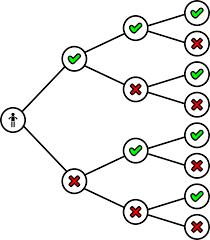
\includegraphics[scale=0.65]{./Imagenes/arbolbin.png}
	\end{figure}		
	\end{columns}
\end{frame}


\begin{frame}{Otra versión}
	\begin{block}{Mejora}
	Forzaremos que la diferencia de jugadores entre ambos equipos no sea mayor de $1$. 
	Si hay un número $n$ par los equipos tendrán el mismo número de jugadores. 
	El algoritmo sigue teniendo eficiencia $O(n)=2^n$ ya que pasaremos por todas las opciones, pero
	cuando una combinación no cumpla dicha restricción no haremos sus cálculos asociados.	
	\end{block}

	\begin{alertblock}{Ajustes}
	El rango usado ha sido $I=[3,26]\cap\mathbb{N}$.
	Hemos ajustado funciones $f(n)=a \cdot 2^n\ a\in\mathbb{R}	\ \forall n\in I$. 
	Sus coeficientes $r^2$ son $1$ en ambos casos (hay pocos elementos) y el 	
	término $a$ está especificado en las gráficas.
	\end{alertblock}
\end{frame}


\subsection{Comparando ambos algoritmos}
\begin{frame}
	\begin{exampleblock}{Sin equilibrio de jugadores}
	\begin{figure}[H]
    		\centering
   		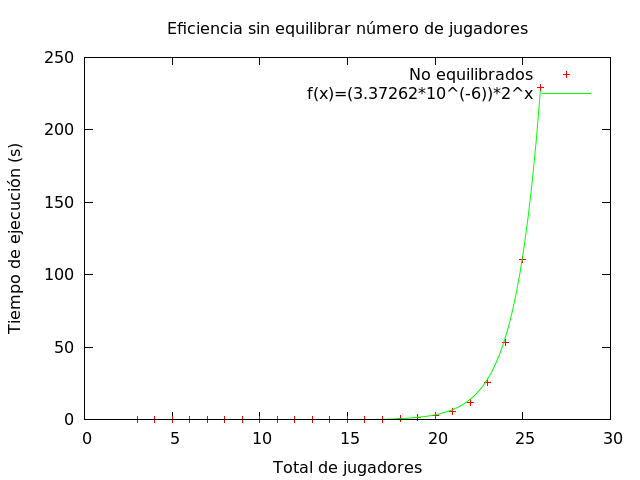
\includegraphics[scale=0.4]{../Equipos/Graficas/sinEquilibrar.png}
    		\label{fig:Sin equilibrar}
	\end{figure}
	\end{exampleblock}
\end{frame}

\begin{frame}
	\begin{exampleblock}{Equilibrando jugadores}
	\begin{figure}[H]
    		\centering
	    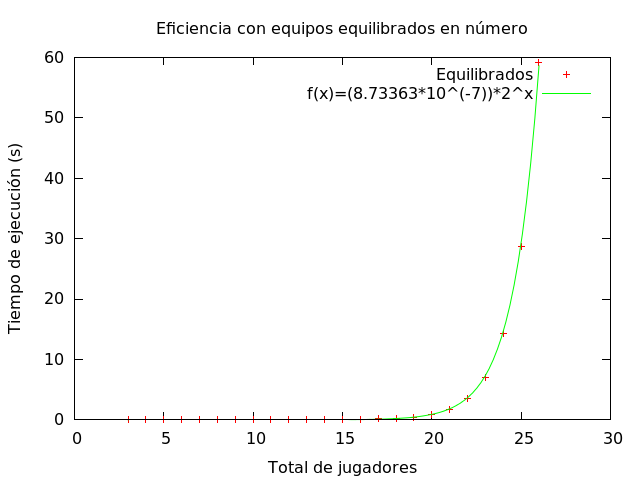
\includegraphics[scale=0.4]{../Equipos/Graficas/equilibrar.png}
    		\label{fig:Equilibrado}
	\end{figure}
	\end{exampleblock}
\end{frame}

\begin{frame}
	\begin{exampleblock}{Comparando tiempo}
	\begin{figure}[H]
    		\centering
	    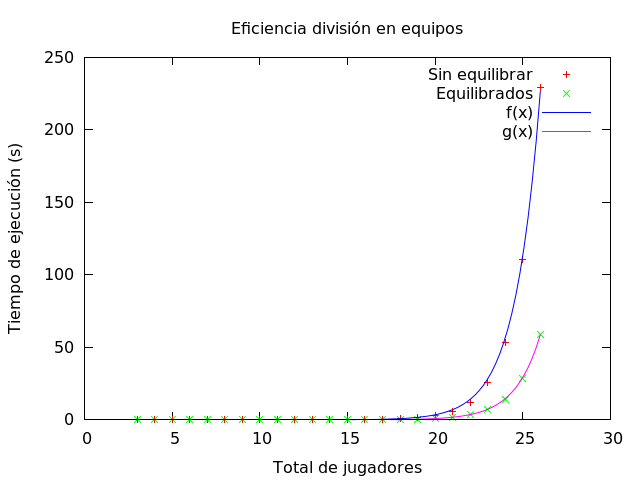
\includegraphics[scale=0.4]{../Equipos/Graficas/tiempos.png}
    		\label{fig:divisionTiempos}
	\end{figure}
	\end{exampleblock}
\end{frame}

\begin{frame}
	\begin{block}{Nivel}
	Recordemos que un jugador tiene un nivel entre $1$ y $1000$, es lógico pensar que con pocos 
	jugadores el margen de optimización del algoritmo es menor debido al gran peso que toma la
	aleatoriedad con la que se determinan los niveles.
	\end{block}
	
	\begin{block}{Tendencia}
	El primer algoritmo tiende a desajustar el número de jugadores, llegando a tener los equipos 
	una diferencia de $4$ jugadores cuando siendo $24$ en total.
	\end{block}
\end{frame}

\begin{frame}
	\begin{exampleblock}{Diferencia de nivel entre los equipos}
		\begin{figure}[H]
    		\centering
    		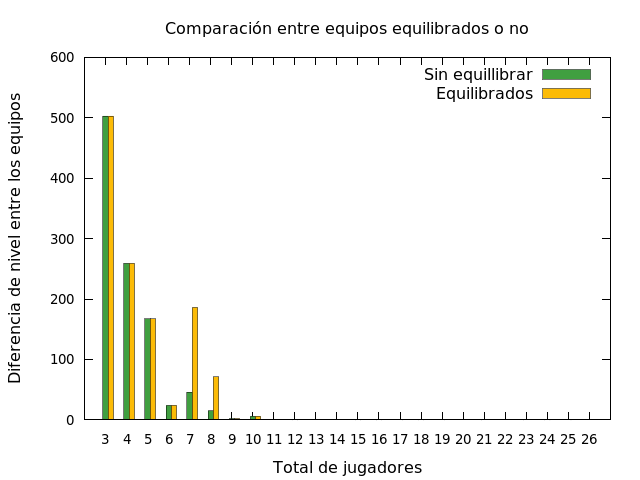
\includegraphics[scale=0.4]{../Equipos/Graficas/comparativa.png}
    		\label{fig:comparativa}
	\end{figure}
	\end{exampleblock}
\end{frame}

\begin{frame}
	\begin{exampleblock}{Número de jugadores de diferencia}
	\begin{figure}[H]
    		\centering
    		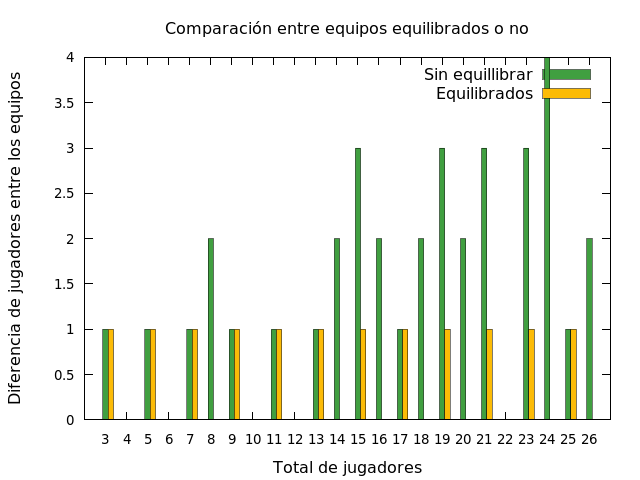
\includegraphics[scale=0.4]{../Equipos/Graficas/separacion.png}
    		\label{fig:separacion}
	\end{figure}
	\end{exampleblock}
\end{frame}

\subsection{Conclusión}
\begin{frame}
	\begin{block}{Opciones}
	Para ejecuciones con un número pequeño de elementos los algoritmos planteados nos sirven, 
	pero si aumentamos el número esa fuerza bruta no es tan buena idea.
	
	Opciones:
	\begin{itemize}
		\item Poda el árbol: ``Branch and Bound".
		\item $x,y$ nivel de los equipos, conformarnos con $|x-y|<n\in\mathbb{N}$
		\item Paralelismo, cada procesador comprueba una rama
	\end{itemize}
	\end{block}
	
	\pause
	\begin{alertblock}{Conclusión}
	Como hemos comprobado, el segundo algoritmo iguala al primero en eficacia, pero lo supera
	en eficiencia.
	Esto nos hace pensar que puede no ser necesario siempre recorrer todo el árbol de soluciones 
	para asegurarnos la optimalidad.
	\end{alertblock}
\end{frame}